\documentclass{tucplain}
\usepackage[ngerman]{babel}
\usepackage[utf8]{inputenc}
\usepackage{amsmath, amssymb, amsfonts}
\usepackage[capitalise, noabbrev]{cleveref}
\usepackage[nolist]{acronym}
\usepackage[colorinlistoftodos]{todonotes}
\usepackage[onehalfspacing]{setspace}
\usepackage{csquotes, titling}


\usetikzlibrary{arrows}
\graphicspath{{images/}}
\bibliographystyle{alpha}
\newgeometry{left=2cm,right=3cm,top=0.5cm,bottom=0.5cm,includeheadfoot}


\newcommand*{\sa}[1]{\todo[color=yellow]{\footnotesize\textbf{@Sven:} #1}}
\newcommand*{\pk}[1]{\todo[color=green]{\footnotesize\textbf{@Phil:} #1}}

\crefname{figure}{Abbildung}{Abbildungen}
\crefname{section}{Kapitel}{Kapitel}

\setlength{\parskip}{0.5em}

\begin{acronym}
    \acro{NaSch-Modell}{Nagel-Schreckenberg-Modell}
    \acro{MAS}{Multi-Agenten System}
    \acro{MASSIM}{Multi-Agenten Simulation}
\end{acronym}


\title{\textbf{Empirischer Vergleich des Multi-Lane-Nagel-Schreckenberg-Fahrzeugfolgemodells mit einem heuristisch basierten Ansatz}}
\author{Sven Albert-Pedersen}
\date{\today}


\begin{document}
    % wir nutzen nicht \ref sondern \cref für Referenzen, hier muss man aber etwas tricksen
    % https://ctan.org/pkg/cleveref
    \let\ref\cref
    
    
    %\listoftodos
    
    \begin{titlingpage}

\begingroup
\begin{figure}[h!]
    \centering
	
\includegraphics[width=0.9\textwidth]{logo}
\end{figure}
\let\newpage\relax%
\center\huge{\textbf{Bachelorarbeit}}
\maketitle
\endgroup

\end{titlingpage}

\tableofcontents
\listoffigures
    \section{Einleitung}
\label{sec:einleitung}


Als Verkehr kann eine Vielzahl verschiedener Arten der Fortbewegung bezeichnet werden. 
Dazu dienen unterschiedliche Verkehrsmittel, mit denen sich an Land, auf dem Wasser oder in der Luft fortbewegt werden kann.
Landbasiert unterscheidet man wiederum in straßen-/wege- oder schienenbasiert.



Laut Statistischem Bundesamt gab es 2016 auf Autobahnen 21193 Unfälle, davon 1435 innerhalb von Baustellen \cite{unf2016}. 
Bei den etwa 13000 km Autobahn \cite{autob2016} entspricht dies durchschnittlich etwa einem Unfall pro 200 km Strecke pro Tag. 
In Wirklichkeit wird es aber Unfallschwerpunkte geben, die diesen Durchschnittswert überschreiten.



 
%Hierfür sind Regeln für Spurwechsel nötig.
%Diese sind fest vorgegeben und werden von jedem \enquote*{Fahrzeugführer} in einer vergleichbaren oder auch nur ähnlichen Situation befolgt.
%
%Dieses simulatorische Verhalten trifft die Realität aber nur bedingt.
%Eine gewisse Anzahl an Fahrern könnte sich, vielleicht aufgrund von Ängsten, Ablenkungen oder auch Fehleinschätzungen, gegen einen Spurwechsel entscheiden, bzw. diesen nicht in Erwägung ziehen.
%Studien zufolge sind drei Viertel der Autofahrer abgelenkt, wenn sie am Steuer sitzen. 
%Jeder zehnte Verkehrsunfall in Deutschland wird durch unaufmerksame Autofahrer verursacht. 
%In Österreich und der Schweiz geht man, aufgrund der Einordnung in eine eigene Kategorie für diese Art Unfälle, von einer Rate von etwa 30\% der Unfälle mit Personenschäden oder gar Toten aus. (vgl. \cite{dvr-studie})
%
%Dieser Verhaltensweise trägt eine theoretische Modellentwicklung in \cite{dat-ba} aus dem Jahr 2017 Rechnung.
%Durch individuelle Berechnungen einer Tendenz zum Fahrspurwechsel, in die die Position und Geschwindigkeit vorausfahrender und nachfolgender Fahrzeuge mit eingehen, und einem stochastisch basierten Wahlprozess könnte es möglich sein, Verhalten, wie sie oben beschrieben wurden, zu simulieren.
%Unterschiedliche Voraussetzungen des Verkehrsgeschehens führen zu unterschiedlichen Wahrscheinlichkeiten und damit zu verschieden hohen Chancen einen Spurwechsel \textit{nicht} durchzuführen.
%
%Es gilt zu klären, ob das theoretische Modell praktisch funktioniert und ob es den Verkehrsfluss realistisch oder sogar realistischer als bisherige Ansätze darstellen kann.
    \section{Problemstellung}
\label{sec:problemstellung}





%% sa{Schreibt das aus \cref{sec:sota} und \cref{sec:researchgap} am Ende zusammen, also im Grunde eine Kurzzusammenfassung von diesen beiden Kapiteln}
%
%Die Simulation von Verkehrsflüssen ist aufgrund des unsicheren Faktors Mensch, der als Haupt"-entscheider nur durch Wahlmöglichkeiten mit vorgegebenen unterschiedlich hohen Wahrscheinlichkeiten modelliert werden kann, ein Bereich in dem seit mehr als sechs Jahrzehnten geforscht wird.
%
%Verschiedene Ansätze, Fahrverhalten zu simulieren, wurden in dieser Zeit verfolgt - Strö"-mungs"-dy"-na"-mik, boolsche Simulation, Zellularautomaten. Letztere werden seit etwa 25 Jahren für die Verkehrssimulation verwendet.
%
%Nagel und Schreckenberg ist es 1992 in \cite{na-sch} gelungen, mit einfachen Regeln das mikroskopische Verhalten jedes Fahrzeugführers so abzubilden, dass sich die makroskopische Sicht auf den Verkehrsfluss realistisch darstellte.
%Erstmals konnte das Entstehen von \enquote{Stau aus dem Nichts} und das Vorhandensein von \enquote{Stauwellen}, die sich rückwärts durch einen solchen Stau bewegen, simulatorisch dargestellt werden.
%
%1995 gelang es mit Hilfe des \enquote{Nagel-Schreckenberg-Modells}, so der heute verwandte und bekannte Name, das gesamte deutsche Autobahnnetz in Echtzeit zu simulieren. 
%Ebenso wird das Modell im Rahmen des Programmes TRANSIMS zur Simulation des Straßenverkehrs der Schweiz eingesetzt. (vgl. \cite{spahn-da})
%
%1996 folgte in \cite{multi-lane} eine Ausdehnung des Modells auf Mehrspurigkeit.  
%Hierfür sind Regeln für Spurwechsel nötig.
%Diese sind fest vorgegeben und werden von jedem \enquote*{Fahrzeugführer} in einer vergleichbaren oder auch nur ähnlichen Situation befolgt.
%
%Dieses simulatorische Verhalten trifft die Realität aber nur bedingt.
%Eine gewisse Anzahl an Fahrern könnte sich, vielleicht aufgrund von Ängsten, Ablenkungen oder auch Fehleinschätzungen, gegen einen Spurwechsel entscheiden, bzw. diesen nicht in Erwägung ziehen.
%Studien zufolge sind drei Viertel der Autofahrer abgelenkt, wenn sie am Steuer sitzen. 
%Jeder zehnte Verkehrsunfall in Deutschland wird durch unaufmerksame Autofahrer verursacht. 
%In Österreich und der Schweiz geht man, aufgrund der Einordnung in eine eigene Kategorie für diese Art Unfälle, von einer Rate von etwa 30\% der Unfälle mit Personenschäden oder gar Toten aus. (vgl. \cite{dvr-studie})
%
%Dieser Verhaltensweise trägt eine theoretische Modellentwicklung in \cite{dat-ba} aus dem Jahr 2017 Rechnung.
%Durch individuelle Berechnungen einer Tendenz zum Fahrspurwechsel, in die die Position und Geschwindigkeit vorausfahrender und nachfolgender Fahrzeuge mit eingehen, und einem stochastisch basierten Wahlprozess könnte es möglich sein, Verhalten, wie sie oben beschrieben wurden, zu simulieren.
%Unterschiedliche Voraussetzungen des Verkehrsgeschehens führen zu unterschiedlichen Wahrscheinlichkeiten und damit zu verschieden hohen Chancen einen Spurwechsel \textit{nicht} durchzuführen.
%
%Es gilt zu klären, ob das theoretische Modell praktisch funktioniert und ob es den Verkehrsfluss realistisch oder sogar realistischer als bisherige Ansätze darstellen kann.
    \section{State-of-the-Art}
\label{sec:sota}







%Bereits seit den 1950er Jahren wurden strömungsdynamische Ansätze für die Simulation von Verkehrsflüssen entwickelt. 
%Außerdem gab es ab den 1980er Jahren auch boolsche Simulationsmodelle, die mit Gitter-Gas-Automaten Flüssigkeiten simulieren konnten.
%Anfang der 1990er wurde von Kai Nagel und Michael Schreckenberg in \cite{na-sch} ein Verfahren vorgestellt, welches Autobahnverkehr basierend auf Zellularautomaten modelliert. 
%
%\begin{quote}
%Ein zellulärer Automat ist eine regelmäßige Annordnung von Zellen. Jede Zelle kann eine endliche Zahl von Werten / Zuständen annehmen und hat eine  begrenzte Zahl von Nachbarzellen, die sie beeinflussen können. Das Muster des gesamten zellulären Automaten ändert sich in einzelnen Schritten, die durch eine Reihe von Übergangsregeln bestimmt werden, die für alle Zellen gelten. (aus \cite{cell-autom})
%\end{quote}
%
%\noindent
%Vereinfacht kann eine Fahrspur einer Straße als Aneinanderreihung vieler solcher Zellen gesehen werden. 
%Dies führt schließlich zu einer gridbasierten Simulationsumgebung. 
%In \cite{na-sch} wird die Rechenumgebung als eindimensionales Array mit $L$ Zellen definiert. 
%Jede der Zellen kann entweder von einem Fahrzeug belegt oder frei sein. 
%Eine Simulation in dieser Grid-Welt hat den Vorteil, dass die Erkenntnisse auf die reale Welt skaliert werden können. 
%Es wird eine Zelllänge von 7,5\nolinebreak[4] m angenommen (vgl. \cite[S. 2227]{na-sch}), was ungefähr dem beanspruchten Platz eines Pkw - von Fahrzeugfront zu Fahrzeugfront - in einer Stausituation entspricht (Fahrzeuglänge + Abstand). 
%Jedes Fahrzeug hat eine ganzzahlige Geschwindigkeit zwischen null und $v_{max}$.
%
%\begin{table}[ht]
%\begin{center}
%\setlength{\tabcolsep}{0.5em} % for the horizontal padding
%{\renewcommand{\arraystretch}{1.2}% for the vertical padding
%\begin{tabular}{| c | c | c |}
%\hline 
%$v^{sim}$ in $\frac{Zellen}{Zeitschritt}$ & $\widehat{=}$ $v^{real}$ in $\frac{m}{s}$ & $=$ in $\frac{km}{h}$ \\ \hline 
%$1$ & 7,5 & 27 \\ \hline
%$2$ & 15 & 54 \\ \hline
%$3$ & 22,5 & 81 \\ \hline
%$4$ & 30 & 108 \\ \hline
%$5$ & 37,5 & 135 \\ \hline
%$6$ & 45 & 162 \\ \hline
%\end{tabular}
%}
%\caption{Umrechnung Geschwindigkeiten Gridwelt $\rightarrow$ reale Welt}
%\end{center}
%\label{tab:umrechnung-zelle-kmh}
%\end{table}
%
%\noindent
%Die beobachtete Durchschittsgeschwindigkeit von 4,5 Zellen/Zeitschritt, der als eine Sekunde angenommen wird, entspricht etwa der einer Geschwindigkeit von 120 km/h (vgl. \cite[S. 2227]{na-sch}). 
%
%In \cite{na-sch} war es erstmals gelungen, Wechselwirkungen zwischen Fahrzeugen im Einspurfall darzustellen und u. a. das Entstehen von Staus, ohne dass ein Grund dafür vorlag, zu modellieren. 
%Mit drei Regeln, die auf jedes Fahrzeug gleichzeitig und gleichermaßen anzuwenden waren, wurde ein realistischer Verkehrsfluss generiert. 
%Die folgenden Regeln, die die Kollisionsfreiheit sichern, sind die Grundlage für die, heute als \enquote{Nagel-Schreckenberg-Modell} bekannte, Modellierung:
%
%\begin{itemize}
%\item \textit{Beschleunigung}: Solange ein Fahrzeug nicht seine max. Geschwindigkeit $v_{max}$ (Zellen/""Zeitschritt) erreicht hat und ein vorausfahrendes Fahrzeug weit genug entfernt ist, erhöht es die Geschwindigkeit um $1$, $v \rightarrow v+1$;
%\item \textit{Abbremsen}: Hat ein Fahrzeug ein anderes Fahrzeug $j$ Zellen vor sich, dann reduziert es die Geschwindigkeit auf $j-1$, $v \rightarrow j-1$;
%\item Zufallsgröße, auch \textit{\enquote*{Trödelwahrscheinlichkeit}}: Mit einer Wahrscheinlichkeit $p$ wird die Geschwindigkeit ($v > 0$) eines Fahrzeuges um $1$ reduziert, $v \rightarrow v-1$
%\end{itemize}
%
%\noindent
%Die Anweisungen werden in der angegebenen Reihenfolge - für alle Fahrzeuge gleichzeitig - ausgeführt und jedes Fahrzeug um die entsprechende Anzahl Zellen weiter gesetzt.
%
%Dehnt man dieses Modell aber auf mehrere Fahrspuren aus, stößt es an seine Grenzen, weil die Modellierung von Überholvorgängen, bzw. genauer gesagt für das \enquote{Ausscheren} und \enquote{Einscheren}, nicht Teil des ursprünglichen Modells ist. 
%\cite{multi-lane} liefert eine \enquote*{multi-lane}-Betrachtung, wobei die ursprünglichen drei Regeln durch weitere ergänzt wurden, die zum einen ein Auffahren des Nachfolgeverkehrs auf den Spurwechsler und zum anderen auch des die Spur wechselnden auf vorausfahrende Fahrzeuge verhindern. \\
%In der Betrachtung, ob die Aktualisierung der Fahrzeuge parallel oder sequentiell erfolgen soll, wurde erkannt, dass dies für das entwickelte Modell nur geringe Unterschiede macht, da die Rate der Spurwechsel mit den festgelegten Regeln eher gering ist. \\
%Gleichzeitig wurde auch beobachtet, dass Fahrzeuge nicht wieder von der Überholspur in die Normalspur wechselten. Dies wurde mit weiteren Regeln und einer Spurwechselwahrscheinlichkeit abgestellt. Eine weitere Kalibrierung des Modells wurde in einer Folgearbeit durchgeführt. \\
%Durch die Konstanthaltung der Anzahl generierter Fahrzeuge und die Veränderung der Systemgröße konnten verschiedene Verkehrsdichten simuliert werden.
%
%\cite{multi-lane} zeigt mehrere Diagramme. Eine Untersuchung von realen Spurwechselvorgängen ergab, dass eine Umkehr der Benutzungshäufigkeit der rechten und linken Spuren bei einem Verkehrsfluss $q_{12}$ von etwa 1200 (Fahrzeugen) pro Stunde auf beiden Spuren erfolgt.
%
%Die Simulation ergab, dass der Punkt, an dem beide Spuren gleichermaßen benutzt werden, deutlich unter dem Punkt liegt, an dem der maximale Verkehrsfluss erreicht wird, siehe \cref{figure:verkehrsfluss-spurnutzung}.
%
%\begin{figure}[hptb]
% \centering
% 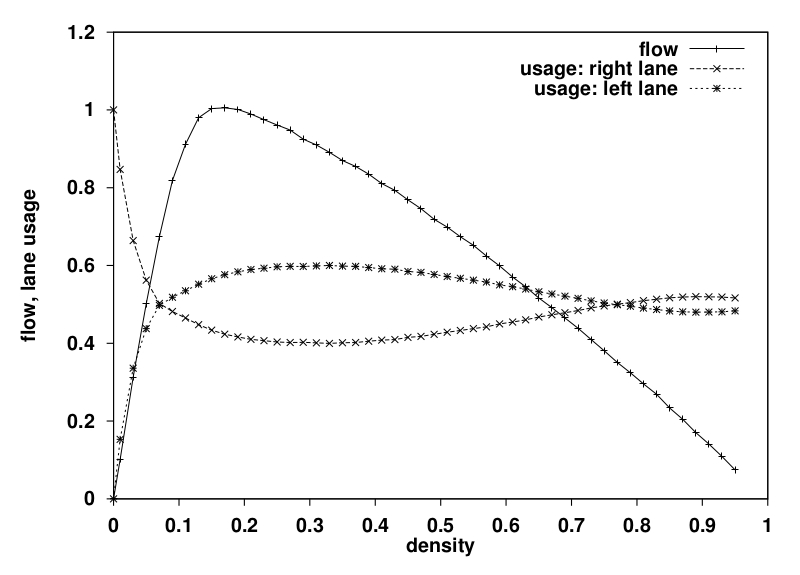
\includegraphics[width=0.7\textwidth]{verkehrsfluss-spurnutzung}
% \caption[Verkehrsfluss und Spurnutzung als Funktion der Verkehrsdichte]{Verkehrsfluss und Spurnutzung als Funktion der Verkehrsdichte, aus \cite{multi-lane}}
% \label{figure:verkehrsfluss-spurnutzung}
%\end{figure}
%
%\noindent
%Ein weiteres Resultat der Simulation ist eine mehrfache Umkehr der Nutzung der Fahrspuren abhängig von der Verkehrsdichte, wenn andere Parameter konstant gehalten werden, siehe \cref{figure:verkehrsfluss}.
%
%\begin{figure}[hptb]
% \centering
% 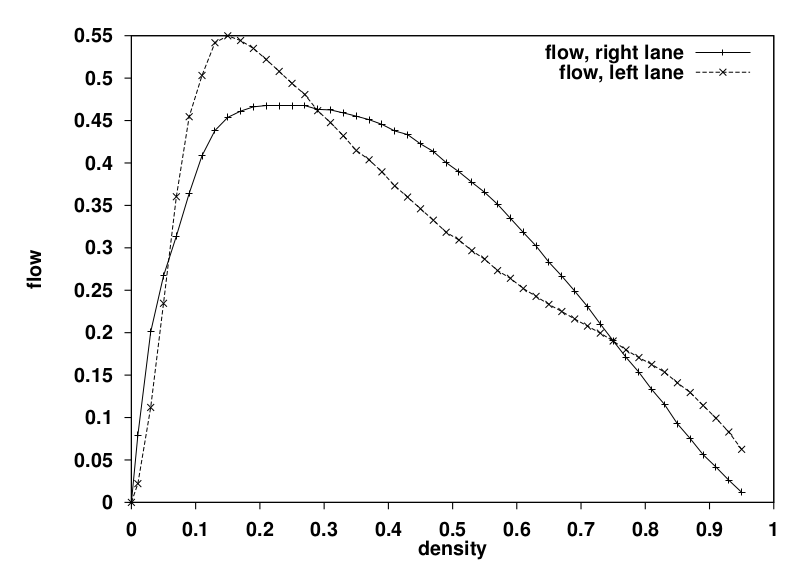
\includegraphics[width=0.7\textwidth]{verkehrsfluss}
% \caption[Verkehrsfluss als Funktion der durchschnittlichen Verkehrsdichte]{Verkehrsfluss auf den Fahrspuren als Funktion der durchschnittlichen Verkehrsdichte, aus \cite{multi-lane}}
% \label{figure:verkehrsfluss}
%\end{figure}
%
%\noindent
%Die Festlegung einer Wahrscheinlichkeit für das Zurückwechseln von der linken auf die rechte Fahrspur führte zu einer unterschiedlichen Spurwechselfrequenz, siehe \cref{figure:spurwechselfrequenz}.
%
%\begin{figure}[hptb]
% \centering
% 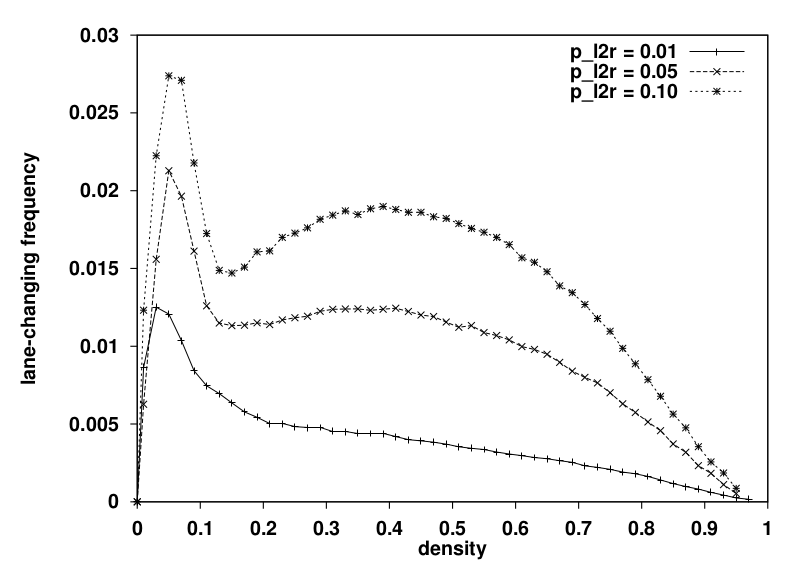
\includegraphics[width=0.7\textwidth]{spurwechselfrequenz}
% \caption[Spurwechselfrequenz als Funktion der Verkehrsdichte]{Spurwechselfrequenz als Funktion der Verkehrsdichte für verschiedene Spurwechselwahrscheinlichkeiten, aus \cite{multi-lane}}
% \label{figure:spurwechselfrequenz}
%\end{figure}
%
%\pagebreak
%In \cite{dat-ba} wurde mit dem \enquote{Social-Force-Vehicle-Modell} ein neuer Ansatz für die Simulation von Spurwechseln entwickelt.
%Auch hier wird eine Grid-Umgebung verwendet.
%Im Gegensatz zur ursprünglichen erdachten Nutzung der \enquote{Social Forces} für Fußgänger, wie z. B. in \cite{soc-for} beschrieben, wird dieses System auf die Gridzellen angewandt. Die Kräfte der Zellen, siehe \cref{figure:social-forces}, werden für jedes Fahrzeug zu jedem Zeitschritt $t$ berechnet, da seine Position zum Zeitpunkt $t + 1$ von der Position im vorhergehenden Zeitschritt abhängt.
%Von den ein Fahrzeug umgebenden acht Zellen müssen, aufgrund der Bewegungsrichtung, nur die drei betrachtet werden, die sich in Fahrtrichtung befinden.
%
%\begin{figure}[hptb]
% \centering
% 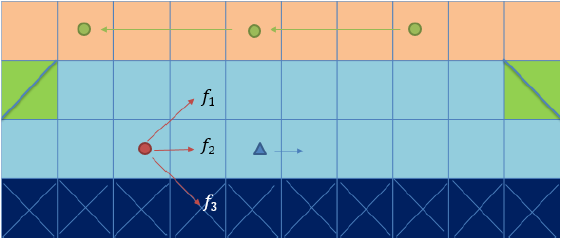
\includegraphics[width=0.7\textwidth]{social-forces}
% \caption[\enquote{Social Forces} für Grid-Zellen]{Vorschlag der \enquote{Social Forces} für Grid-Zellen, aus \cite{dat-ba}}
% \label{figure:social-forces}
%\end{figure}
%
%\noindent
%Die letztendliche Auswahl der Zielzelle wird mittels \enquote{Fitness-proportionate Selection} durchgeführt.
%Entgegen des Zwangs zum Ausscheren und einer fest vorgegebenen Wahrscheinlichkeit wird eine stochastische Simulationsmöglichkeit der Neigung zum Spurwechsel aufgezeigt. 
%    \section{Research Gap}
\label{sec:researchgap}



%In der Multi-Lane-Version des Nagel-Schreckenberg-Modells (siehe \cite{multi-lane}) geben die Regeln einen Zwang zum Einleiten des Überholvorganges, wenn sich die Möglichkeit dazu ergibt, vor. Ebenso wurde für den Rückwechsel auf die Normalspur eine Wahrscheinlichkeit festgelegt.
%
%Das Verhalten des Entscheiders Mensch, was auch im Straßenverkehr eine große Rolle spielt, wurde bisher eher als eine Art \enquote{Black Box} betrachtet. 
%Jeder Fahrzeugführer trifft zu jedem Zeitpunkt unter gleichen Voraussetzungen die gleiche Entscheidung. 
%Dies ist aber in der Realität nicht so. 
%Ein Fahrer kann z. B. vorsichtiger sein als ein anderer und, trotz des gleichen Abstands und der gleichen Geschwindigkeiten, auf ein Überholmanöver verzichten, weil er seine Umwelt anders einschätzt.
%
%In \cite{dat-ba} wird der Hang zum Wechsel oder zur Beibehaltung der Spur nicht nur durch fest vorgegebene Wahrscheinlichkeiten simuliert, sondern durch individuell für jedes Fahrzeug zu jedem Zeitschritt berechnete \enquote{Kräfte}, deren \enquote*{Entscheidung}, durch entsprechende berechnete Wahrscheinlichkeiten getragen, mehr oder weniger häufig zur Ausführung kommen. 
%Durch die gezielte Beachtung des umgebenden Verkehrs und das Bewerten der zur Wahl stehenden Alternativen soll es nun möglich sein, das menschliche Verhalten besser als bisher abzubilden.
%
%Das Hauptaugenmerk von \cite{dat-ba} lag auf der theoretischen Modellentwicklung/""Modellierung. 
%Eine praktische Umsetzung und somit die Kontrolle des Erdachten und natürlich die Möglichkeit eines Vergleichs zwischen dem neuen Ansatz und bereits existierenden Modellierungen, z. B. dem Mehrspurmodell aus \cite{multi-lane}, ist bisher nicht durchgeführt worden. 
%Dies ist Ziel dieser Arbeit.
%
%\subsection*{Mögliches Problem}
%\addcontentsline{toc}{subsection}{Mögliches Problem}
%
%Aus der Art und Weise, wie der Ansatz in das ursprüngliche Modell nach \cite{na-sch} (und nicht in die Mehrspurvariante nach \cite{multi-lane}) integriert wurde, könnte ein Problem entstehen.
%Eine der drei Regeln, die die Kollisionsfreiheit sichern sollen - das Abbremsen - wurde entfernt und durch das \enquote{Social-Force-Modell} ersetzt (siehe \cite{dat-ba}, S. 21 \& Abb. 16, bzw. Vortragsfolien S. 7).
%Dies kann dazu führen, dass in der Simulation ein Auffahrunfall unausweichlich ist.
%Auch wenn Verkehrsunfälle in der realen Welt durchaus vorkommen, sollte man sie in dieser Simulation nicht provozieren. Zudem ist die Unfallhäufigkeit so gering, dass sie bei betrachteter Zeitspanne und Streckenlänge unbedeutend ist.
%
%\begin{figure}[hptb]
% \centering
% 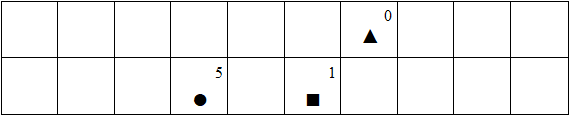
\includegraphics[width=0.6\textwidth]{problem-beispiel}
% \caption[Problem-Beispiel]{Beispiel für ein Problem-Szenario, drei Fahrzeuge und deren Geschwindigkeiten}
% \label{figure:problem-beispiel}
%\end{figure}
%
%\noindent
%In \cref{figure:problem-beispiel} würde dem Fahrzeug $\bullet$ nach dem Multi-Lane-Modell aus \cite{multi-lane} das Ausscheren vorgegeben, denn die linke Spur bietet mehr Platz als die rechte und es gibt keinen nachfolgenden Verkehr auf der anderen Spur. 
%Fahrzeug $\blacktriangle$ ist $j=3$ Felder vor $\bullet$.
%Ein Abbremsen von $\bullet$ auf $v_{\bullet}=j-1=2$ würde veranlasst.
%Dass $\blacktriangle$ gleichzeitig um $1$ beschleunigen könnte, spielt keine Rolle. \\
%Nach dem \enquote{Social-Force-Modell} würde für das Fahrzeug $\bullet$ wahrscheinlich eine höhere Kraft der entsprechenden Zelle und somit Wahrscheinlichkeit für das Ausscheren berechnet werden.
%Dies muss aber nicht zur Entscheidung in Richtung Spurwechsel führen.
%$\blacksquare$ kann im aktuellen Zeitschritt max. auf $v_{\blacksquare}=2$ beschleunigen, $\blacktriangle$ max. auf $v_{\blacktriangle}=1$.
%Da Fahrzeug $\bullet$ seine Geschwindigkeit aber nur durch die Zufallsgröße \enquote{Trödeln} um max. $1$ reduzieren könnte, würde es beim Simulationsschritt \enquote{Fahren} auf das gleiche Grid-Feld oder gar davor gesetzt werden. \\
%Da ein solches Szenario insbesondere bei Stockungen und an Stauenden auftreten dürfte, wären dort Auffahrunfälle unvermeidbar. 
%
%Das \enquote{Social-Force-Modell} wird im normalen Verkehrsfluss einen Teil der möglichen Unfallszenarien durch Ausweichen verhindern, aber bei \enquote*{Auswahl} der weniger wahrscheinlichen Alternative geradeaus zu fahren, wird sich das fehlende \enquote*{Bremsen} bemerkbar machen.

%    \section{Vorläufige Realisierung}
\label{sec:realisierung}







%%.\sa{hier vermischst Du \cref{sec:sota} mit \cref{sec:realisierung}, hier geht es darum, wi Du konkret arbeiten willst um die Sachen unter \cref{sec:researchgap} zu beweisen oder zu belegen, evtl macht es Sinn diese Punkte mit in \cref{sec:sota} zu ziehen, Du kannst dann einfach, wenn Du es brauchst Verweise setzen}
%
%\noindent
%Die in \cite{dat-ba} vorgeschlagene Struktur ist zu implementieren und in vergleichbarer Umgebung simulatorisch zu testen. 
%Dabei sind die folgenden Größen zu erheben und entsprechend statistisch auszuwerten: 
%
%\begin{itemize}
%\item Verkehrsdichte
%\item Verkehrsfluss
%\item Spurwechselfrequenz
%\item Spurnutzung links/rechts
%\end{itemize}
%
%Das Testszenario wurde in \cite{na-sch} durch das zu Beginn zufällige Platzieren von Fahrzeugen in einem geschlossenen Kreis mit $L$ Zellen (ähnlich einer Autorennstrecke) simuliert. \\
%Allerdings wurde auch, bei der Simulation einer Fahrbahnverengung, eine Alternative Simulationsmöglichkeit beschrieben. 
%Eine Gridgerade von bis zu 10000 Zellen Länge wurde getestet - Bewegungsrichtung von links nach rechts. 
%Die Fahrzeuge wurden mit $v=0$ in die am weitesten links befindliche Zelle, so diese frei war, gesetzt und die Fahrzeuge in den sechs am weitesten rechts befindlichen Zellen (bei systemweiter $v_{max}=5$) gelöscht. 
%Letzteres Vorgehen sorgte für eine offene Grenze für den abfließenden Verkehr.
%
%Für eine kontinuierliche Simulation ist die zweite Möglichkeit ungeeignet. 
%Auch in \cite{multi-lane} wird von der Nutzung periodischer Randbedingungen gesprochen. 
%Dies lässt darauf schließen, dass, wie in \cite[Abb. 1.5]{peri-rand} für die Umgebung von Pixeln beschrieben, die Fahrzeuge vom \enquote*{Ende} der Gridstrecke am \enquote*{Anfang} wieder eingesetzt wurden und somit der zuerst beschriebene Kreis einsteht.
%Dieses Verhalten ist zu bevorzugen.
%
%Vorteil der geschlossenen Kreisstrecke ist, dass man bei konstanter Fahrzeuganzahl $N$ (bei \cite{multi-lane} waren dies $N = 10^{3}$) durch die Veränderung der Systemgröße eine unterschiedliche Fahrzeugdichte erreicht werden kann. 
%Jeder Dichtewert wurde für $T = 10^{5}$ Zeitschritte simuliert, wobei die erste Hälfte verworfen wurde, um mögliche Störeffekte ausklingen zu lassen. 
%Die generierten Simulationsdaten wurden über $T_{sample} = 300$ Zeitschritte und eine Wegstrecke von 133 Zellen, was etwa 1 km Länge in der realen Welt entspricht, gemittelt, um statistische Schwankungen zu reduzieren.
%
%Ein mögliches Simulationstool ist das \enquote{Traffic Simulation Game}\footnote{\link{https://lightjason.github.io/news/2017-09-workshop/}}. 
%In der Grundkonfiguration erzeugt dieses eine beliebig lange, gerade Straße mit beliebig vielen Fahrspuren. 
Es ist zu prüfen, ob die Software auf die gewünschte Verhaltensweise angepasst werden kann.
    
    \bibliography{references}

\end{document}

